

%*******************************************************
% This program is free software: you can redistribute it and/or modify
% it under the terms of the GNU General Public License as published by
% the Free Software Foundation, either version 3 of the License, or
% (at your option) any later version.
%
% This program is distributed in the hope that it will be useful,
% but WITHOUT ANY WARRANTY; without even the implied warranty of
% MERCHANTABILITY or FITNESS FOR A PARTICULAR PURPOSE.  See the
% GNU General Public License for more details.
%
% You should have received a copy of the GNU General Public License
% along with this program.  If not, see <http://www.gnu.org/licenses/>.
%*******************************************************
% PhD Thesis Template
% Use XeLatex to typeset
% This template has been tested on
% MacTeX-2015 Distribution
% OS X EI Capitan version 10.11.4
%*******************************************************
% The font is 11pt. Paper size is A4. To be printed
% twoside
%*******************************************************

\documentclass[twoside,paper=a4,fontsize=11pt]{report}

%*******************************************************
% From page 7 of Preparing and Submitting Your
% Thesis - A guide for MPhil and PhD students:
% The thesis submitted for examination shall be typewritten
% or printed on one side or both sides of International size
% A4 paper (except for drawings, maps or tables on
% which no restriction is placed), with a margin of
% not less than 35mm on both right and left-hand
% edges of each page.
% There is no stipulation for the top and bottom margins,
% but it is recommended that they should be 25mm.
% From page10:
% Font heights are usually measured in points and
% the most easily readable fonts are 10 point and 12 point.
%*******************************************************

\usepackage[left=37mm,right=37mm,top=27mm,bottom=27mm]{geometry}

%*******************************************************
% The following three lines set Chinese fonts so that you can
% type your Chinese name.
% The typeset method (so called compiling) is XeLatex.
% Use the Chinese font available on your own computer.
% Yuanti TL Light may not be available on your own computer.
% The scale=1 sets the height of the Chinese font.
%*******************************************************

\usepackage{xeCJK}
\usepackage{fontspec}
\setCJKmainfont[Scale=1]{Yuanti TC Light}

%*******************************************************
% The following two lines set the English fonts
%*******************************************************

\setromanfont{Times New Roman}
\setsansfont{Arial}

%*******************************************************
% Include packages that you wish to use.
%*******************************************************

\usepackage{tikz}
\usetikzlibrary{shapes,arrows}

\usepackage{lipsum} % this generates dummy text

\usepackage{multicol} % use multicolumn
\usepackage{rotating} % to create a figure in landscape mode

\usepackage{natbib} % this is for bibliography
\usepackage{setspace} % this is for setting line spacing

\usepackage{longtable} % this is for longtable


\usepackage{array}


\usepackage{amsthm}
\usepackage{amsmath}
\usepackage{calc}
\usepackage{float}
\usepackage{graphicx}
\usepackage{setspace}
\usepackage{url}

%*******************************************************
% Define hyphenation for some special words
%*******************************************************

\usepackage{hyphenat} % this define hyphenation, an example is given in the next four lines.
\hyphenation{pro-ban-da}
\hyphenation{pro-ban-dum}
\hyphenation{pen-ul-ti-mate}
\hyphenation{sche-ma-tic}

%*******************************************************
% Make "clickable" Table of Contents
%*******************************************************
\usepackage{color}   %May be necessary if you want to color links
\usepackage{hyperref}
\hypersetup{
    %colorlinks=true, %set true if you want colored links
    colorlinks=false
    linktoc=all,         %set to all if you want both sections and subsections linked
    linkcolor=black,  %choose some color, e.g. blue, if you want links to stand out
    }

%*******************************************************
% This is the start of the thesis
%*******************************************************

\begin{document}

\linespread{1.2} % change it to 1 becomes single line spacing. Change it to 1.5 is a half line spacing.

%*******************************************************
% From page 10 of Preparing and Submitting Your Thesis
% A guide for MPhil and PhD students:
% Modern word processing programs will automatically
% adjust the line spacing to match the size of text on any line.
% Single line spacing will produce a dense but readable
% text: the text may seem less formidable if one and a
% spacing is used. Double spacing results in a rather
% empty looking page and significantly increases
% the number of pages in a thesis.
%*******************************************************

%*******************************************************
% These are front matters.
% Abstract
% Title page
% Dedication
% Declaration
% Acknowledgment
% Publication (Optional)
% Table of Contents (Including List of Tables and List of Figures)
%*******************************************************



%*******************************************************
% This program is free software: you can redistribute it and/or modify
% it under the terms of the GNU General Public License as published by
% the Free Software Foundation, either version 3 of the License, or
% (at your option) any later version.
%
% This program is distributed in the hope that it will be useful,
% but WITHOUT ANY WARRANTY; without even the implied warranty of
% MERCHANTABILITY or FITNESS FOR A PARTICULAR PURPOSE.  See the
% GNU General Public License for more details.
%
% You should have received a copy of the GNU General Public License
% along with this program.  If not, see <http://www.gnu.org/licenses/>.
%*******************************************************
% Titlepage
%*******************************************************
\begin{titlepage}
	\begin{center}
	
	Abstract of thesis entitled\\
	
	 \bigskip 
	   	
        \huge\textsc{\textbf{This is the title of my thesis}} \\
            
        \bigskip
        	
        {\normalsize Submitted by}\\
			
	\bigskip  	
        
        \Large{\textbf{Yufen CHUN}}\textbf{淳于棼}\\
       
	\bigskip
	       
	{\normalsize
	for the degree of Doctor of Philosophy\\
	at The University of Hong Kong\\
	in Month Year\\}
        
        \end{center}    
	
	\bigskip
	
	These are the motivations. \lipsum[1]
	
	These are the methods. \lipsum[1]
	
	These are the results. \lipsum[1]
	
	These are the discussions. \lipsum[1]
	
	These are the significance. \lipsum[1]
	
	\bigskip
	
	\begin{center}
	
	\rule{6cm}{0.025cm}\\
	{\slshape An abstract of exactly 499 words}
	
	\end{center}  
\end{titlepage}   


\cleardoublepage



%*******************************************************
% This program is free software: you can redistribute it and/or modify
% it under the terms of the GNU General Public License as published by
% the Free Software Foundation, either version 3 of the License, or
% (at your option) any later version.
%
% This program is distributed in the hope that it will be useful,
% but WITHOUT ANY WARRANTY; without even the implied warranty of
% MERCHANTABILITY or FITNESS FOR A PARTICULAR PURPOSE.  See the
% GNU General Public License for more details.
%
% You should have received a copy of the GNU General Public License
% along with this program.  If not, see <http://www.gnu.org/licenses/>.
%*******************************************************
% Titlepage
%*******************************************************
\begin{titlepage}
	\begin{center}
		\large  
	        \hfill
	        \vfill
        \begingroup
            \huge\textsc{\textbf{This is the title of my thesis}} \\
            \bigskip
        \endgroup
         by\\
	\bigskip  	
        \Large\textsc{\textbf{Yufen CHUN}}\\
						\textbf{淳于棼}
        \vfill
        \vfill
        \vfill
	{\normalsize
	A thesis submitted in partial fulfilment of the requirements for\\
	the Degree of Doctor of Philosophy\\
	at The University of Hong Kong.\\
		\bigskip
	Month Year}
        \vfill                      
    	\end{center}      
\end{titlepage}   


\cleardoublepage



%*******************************************************
% This program is free software: you can redistribute it and/or modify
% it under the terms of the GNU General Public License as published by
% the Free Software Foundation, either version 3 of the License, or
% (at your option) any later version.
%
% This program is distributed in the hope that it will be useful,
% but WITHOUT ANY WARRANTY; without even the implied warranty of
% MERCHANTABILITY or FITNESS FOR A PARTICULAR PURPOSE.  See the
% GNU General Public License for more details.
%
% You should have received a copy of the GNU General Public License
% along with this program.  If not, see <http://www.gnu.org/licenses/>.
%*******************************************************
% Dedication
%*******************************************************
\thispagestyle{empty}

\vspace*{3cm}
\vspace*{2cm}

\begin{center}
This thesis is dedicated to those to whom you wishes to dedicate.
\end{center}


\cleardoublepage

\pagenumbering{roman}

\pagestyle{plain}



%*******************************************************
% This program is free software: you can redistribute it and/or modify
% it under the terms of the GNU General Public License as published by
% the Free Software Foundation, either version 3 of the License, or
% (at your option) any later version.
%
% This program is distributed in the hope that it will be useful,
% but WITHOUT ANY WARRANTY; without even the implied warranty of
% MERCHANTABILITY or FITNESS FOR A PARTICULAR PURPOSE.  See the
% GNU General Public License for more details.
%
% You should have received a copy of the GNU General Public License
% along with this program.  If not, see <http://www.gnu.org/licenses/>.
%*******************************************************
% Declaration
%*******************************************************

\addcontentsline{toc}{chapter}{Declaration}%% to be removed

\chapter*{Declarations}

I declare that this thesis represents my own work, except where due acknowledgement is made, and that it has not been previously included in a thesis, dissertation or report submitted to this University or to any other institution for a degree, diploma or other qualifications.% This is copied from the declaration statement from the Handbook.

\bigskip
\bigskip
\bigskip
\bigskip
\bigskip
\bigskip
\bigskip
\bigskip

\begin{flushright}
    \begin{tabular}{p{1cm} p{4cm}}
        Signed & \dotfill \\
           & \center Yufen CHUN\\
    \end{tabular}
\end{flushright}

\bigskip
\bigskip
\bigskip


\cleardoublepage


%*******************************************************
% This program is free software: you can redistribute it and/or modify
% it under the terms of the GNU General Public License as published by
% the Free Software Foundation, either version 3 of the License, or
% (at your option) any later version.
%
% This program is distributed in the hope that it will be useful,
% but WITHOUT ANY WARRANTY; without even the implied warranty of
% MERCHANTABILITY or FITNESS FOR A PARTICULAR PURPOSE.  See the
% GNU General Public License for more details.
%
% You should have received a copy of the GNU General Public License
% along with this program.  If not, see <http://www.gnu.org/licenses/>.
%*******************************************************
% Acknowledgments
%*******************************************************

\addcontentsline{toc}{chapter}{Acknowledgments}%% to be removed

\chapter*{Acknowledgments}

\begin{flushright}
{\slshape Lorem ipsum dolor sit amet, consectetuer adipiscing.}\\
{\slshape Aenean commodo ligula eget dolor. Aenean massa.}\\% This is a set of dummy text.
\medskip
--- John Doe (1914).% This is a dummy author only.
\end{flushright}

\bigskip

\lipsum[2-5]% This command generate dummy text. Remove this line and replace it by your words of appreciation.



\cleardoublepage


%*******************************************************
% This program is free software: you can redistribute it and/or modify
% it under the terms of the GNU General Public License as published by
% the Free Software Foundation, either version 3 of the License, or
% (at your option) any later version.
%
% This program is distributed in the hope that it will be useful,
% but WITHOUT ANY WARRANTY; without even the implied warranty of
% MERCHANTABILITY or FITNESS FOR A PARTICULAR PURPOSE.  See the
% GNU General Public License for more details.
%
% You should have received a copy of the GNU General Public License
% along with this program.  If not, see <http://www.gnu.org/licenses/>.
%*******************************************************
% Publication
% Generally, this is necessary if your thesis is organised as a
% series of papers.
% Some say this is optional even though their theses are
% organised as a series of papers.
%*******************************************************
\addcontentsline{toc}{chapter}{Publications}%% to be removed

\chapter*{Publications}

Publications arising from this thesis:

\begin{enumerate}
\item Student and Teacher (2015). The title of the work. {\slshape The name of the journal}, 5(3):123-143. (part of Chapter 2 and part of Chapter 3)
\item Student, Dick and Harry (2016). The title of the work.   {\slshape The name of the journal}, 6(8):1123-1143. (part of Chapter 2 and part of Chapter 4)
\end{enumerate}


\cleardoublepage


%*******************************************************
% This program is free software: you can redistribute it and/or modify
% it under the terms of the GNU General Public License as published by
% the Free Software Foundation, either version 3 of the License, or
% (at your option) any later version.
%
% This program is distributed in the hope that it will be useful,
% but WITHOUT ANY WARRANTY; without even the implied warranty of
% MERCHANTABILITY or FITNESS FOR A PARTICULAR PURPOSE.  See the
% GNU General Public License for more details.
%
% You should have received a copy of the GNU General Public License
% along with this program.  If not, see <http://www.gnu.org/licenses/>.
%*******************************************************
% Table of Contents
%*******************************************************


\setcounter{tocdepth}{2} % <-- 2 includes up to subsections in the ToC
\setcounter{secnumdepth}{3} % <-- 3 numbers up to subsubsections

\tableofcontents 

%*******************************************************
% List of Figures and of the Tables
%*******************************************************

\clearpage

\listoffigures

\cleardoublepage
 
\listoftables

\cleardoublepage


%*******************************************************
% Mainmatter
%*******************************************************

\pagenumbering{arabic}

\cleardoublepage



%*******************************************************
% This program is free software: you can redistribute it and/or modify
% it under the terms of the GNU General Public License as published by
% the Free Software Foundation, either version 3 of the License, or
% (at your option) any later version.
%
% This program is distributed in the hope that it will be useful,
% but WITHOUT ANY WARRANTY; without even the implied warranty of
% MERCHANTABILITY or FITNESS FOR A PARTICULAR PURPOSE.  See the
% GNU General Public License for more details.
%
% You should have received a copy of the GNU General Public License
% along with this program.  If not, see <http://www.gnu.org/licenses/>.
%************************************************
\chapter{Introduction}
\label{ch:introduction}
%************************************************

\begin{flushright}
{\slshape Lorem ipsum dolor sit amet, consectetuer adipiscing.}\\
{\slshape Aenean commodo ligula eget dolor. Aenean massa.}\\
% This generate dummy text. Remove this line and replace by your quote.
\medskip
--- John Doe,\\
Unified Theory of the Important Theories,\\
{\slshape An Important Journal},\\
Vol.~123, pp.~1234--1243, Dec.~2016.\\
\end{flushright}

\bigskip


%\minitoc\nomtcpagenumbers

%\marginpar{\myTitle \myVersion}

\section{Introduction}
\label{sec:ch_1_introduction}

This is a topic sentence followed by explanation, elaboration and examples to introduce the next three subsections. The last sentence of this paragraph shall introduce the next paragraph. \lipsum[1]

This is a topic sentence followed by explanation, elaboration and examples to introduce the next three subsections. The last sentence of this paragraph shall introduce the next paragraph. \lipsum[1]

This is a topic sentence followed by explanation, elaboration and examples to introduce the next three subsections. The last sentence of this paragraph shall introduce the next paragraph. \lipsum[1]

\section{Thesis statement and motivation}
\label{sec:ch_1_firstmain}

This is a topic sentence followed by explanation, elaboration and examples to introduce this paragraph. The last sentence of this paragraph shall introduce the next paragraph. \lipsum[1]

This is a topic sentence followed by explanation, elaboration and examples to introduce this paragraph. The last sentence of this paragraph shall introduce the next paragraph. \lipsum[1]

This is a topic sentence followed by explanation, elaboration and examples to introduce this paragraph. The last sentence of this paragraph shall introduce the next paragraph. \lipsum[1]

\section{Research goals and approaches}
\label{sec:ch_1_secondmain}

This is a topic sentence followed by explanation, elaboration and examples to introduce this paragraph. The last sentence of this paragraph shall introduce the next paragraph. \lipsum[1]

This is a topic sentence followed by explanation, elaboration and examples to introduce this paragraph. The last sentence of this paragraph shall introduce the next paragraph. \lipsum[1]

This is a topic sentence followed by explanation, elaboration and examples to introduce this paragraph. The last sentence of this paragraph shall introduce the next paragraph. \lipsum[1]

\section{Contributions}
\label{sec:ch_1_thirdmain}


This is a topic sentence followed by explanation, elaboration and examples to introduce this paragraph. The last sentence of this paragraph shall introduce the next paragraph. \lipsum[1]

This is a topic sentence followed by explanation, elaboration and examples to introduce this paragraph. The last sentence of this paragraph shall introduce the next paragraph. \lipsum[1]

This is a topic sentence followed by explanation, elaboration and examples to introduce this paragraph. The last sentence of this paragraph shall introduce the next paragraph. \lipsum[1]

\section{Thesis organisation}
\label{sec:ch_1_conclusion}


This is a topic sentence followed by explanation, elaboration and examples to summarise the second subsection. The last sentence of this paragraph shall introduce the next paragraph. \lipsum[1]

This is a topic sentence followed by explanation, elaboration and examples to summarise the third subsection. The last sentence of this paragraph shall introduce the next paragraph. \lipsum[1]

This is a topic sentence followed by explanation, elaboration and examples to summarise the fourth subsection. The last sentence of this paragraph shall introduce the next chapter. \lipsum[1]



%*****************************************
%*****************************************
%*****************************************
%*****************************************
%*****************************************






\cleardoublepage



%*******************************************************
% This program is free software: you can redistribute it and/or modify
% it under the terms of the GNU General Public License as published by
% the Free Software Foundation, either version 3 of the License, or
% (at your option) any later version.
%
% This program is distributed in the hope that it will be useful,
% but WITHOUT ANY WARRANTY; without even the implied warranty of
% MERCHANTABILITY or FITNESS FOR A PARTICULAR PURPOSE.  See the
% GNU General Public License for more details.
%
% You should have received a copy of the GNU General Public License
% along with this program.  If not, see <http://www.gnu.org/licenses/>.
%************************************************
\chapter{Literature review}
\label{ch:name2}
%************************************************

\begin{flushright}
{\slshape Lorem ipsum dolor sit amet, consectetuer adipiscing.}\\
{\slshape Aenean commodo ligula eget dolor. Aenean massa.}\\
% This generate dummy text. Remove this line and replace by your quote.
\medskip
--- John Doe,\\
Unified Theory of the Important Theories,\\
{\slshape An Important Journal},\\
Vol.~123, pp.~1234--1243, Dec.~2016.\\
\end{flushright}

\bigskip


%\minitoc\nomtcpagenumbers

%\marginpar{\myTitle \myVersion}

\section{Introduction}
\label{sec:ch_2_introduction}

This is a topic sentence followed by explanation, elaboration and examples to introduce the next three subsections. The last sentence of this paragraph shall introduce the next paragraph. \lipsum[1]

This is a topic sentence followed by explanation, elaboration and examples to introduce the next three subsections. The last sentence of this paragraph shall introduce the next paragraph. \lipsum[1]

This is a topic sentence followed by explanation, elaboration and examples to introduce the next three subsections. The last sentence of this paragraph shall introduce the next paragraph. \lipsum[1]

\section{First main stuff}
\label{sec:ch_2_firstmain}


This is a topic sentence followed by explanation, elaboration and examples to introduce this paragraph. The last sentence of this paragraph shall introduce the next paragraph. \lipsum[1]

This is a topic sentence followed by explanation, elaboration and examples to introduce this paragraph. The last sentence of this paragraph shall introduce the next paragraph. \lipsum[1]

This is a topic sentence followed by explanation, elaboration and examples to introduce this paragraph. The last sentence of this paragraph shall introduce the next paragraph. \lipsum[1]

\section{Second main stuff}
\label{sec:ch_2_secondmain}

This is a topic sentence followed by explanation, elaboration and examples to introduce this paragraph. The last sentence of this paragraph shall introduce the next paragraph. \lipsum[1]

This is a topic sentence followed by explanation, elaboration and examples to introduce this paragraph. The last sentence of this paragraph shall introduce the next paragraph. \lipsum[1]

This is a topic sentence followed by explanation, elaboration and examples to introduce this paragraph. The last sentence of this paragraph shall introduce the next paragraph. \lipsum[1]

\section{Third main stuff}
\label{sec:ch_2_thirdmain}

This is a topic sentence followed by explanation, elaboration and examples to introduce this paragraph. The last sentence of this paragraph shall introduce the next paragraph. \lipsum[1]

This is a topic sentence followed by explanation, elaboration and examples to introduce this paragraph. The last sentence of this paragraph shall introduce the next paragraph. \lipsum[1]

This is a topic sentence followed by explanation, elaboration and examples to introduce this paragraph. The last sentence of this paragraph shall introduce the next paragraph. \lipsum[1]

\section{Summary}
\label{sec:ch_2_summary}

This is a topic sentence followed by explanation, elaboration and examples to summarise the second subsection. The last sentence of this paragraph shall introduce the next paragraph. \lipsum[1]

This is a topic sentence followed by explanation, elaboration and examples to summarise the third subsection. The last sentence of this paragraph shall introduce the next paragraph. \lipsum[1]

This is a topic sentence followed by explanation, elaboration and examples to summarise the fourth subsection. The last sentence of this paragraph shall introduce the next chapter. \lipsum[1]



%*****************************************
%*****************************************
%*****************************************
%*****************************************
%*****************************************






\cleardoublepage



%*******************************************************
% This program is free software: you can redistribute it and/or modify
% it under the terms of the GNU General Public License as published by
% the Free Software Foundation, either version 3 of the License, or
% (at your option) any later version.
%
% This program is distributed in the hope that it will be useful,
% but WITHOUT ANY WARRANTY; without even the implied warranty of
% MERCHANTABILITY or FITNESS FOR A PARTICULAR PURPOSE.  See the
% GNU General Public License for more details.
%
% You should have received a copy of the GNU General Public License
% along with this program.  If not, see <http://www.gnu.org/licenses/>.
%************************************************
\chapter{This is chapter three}
\label{ch:name3}
%************************************************

\begin{flushright}
{\slshape Lorem ipsum dolor sit amet, consectetuer adipiscing.}\\
{\slshape Aenean commodo ligula eget dolor. Aenean massa.}\\
% This generate dummy text. Remove this line and replace by your quote.
\medskip
--- John Doe,\\
Unified Theory of the Important Theories,\\
{\slshape An Important Journal},\\
Vol.~123, pp.~1234--1243, Dec.~2016.\\
\end{flushright}

\bigskip

\section{Introduction}
\label{sec:ch_3_introduction}

This is a topic sentence followed by explanation, elaboration and examples to introduce the next three subsections. The last sentence of this paragraph shall introduce the next paragraph. \lipsum[1]

This is a topic sentence followed by explanation, elaboration and examples to introduce the next three subsections. The last sentence of this paragraph shall introduce the next paragraph. \lipsum[1]

This is a topic sentence followed by explanation, elaboration and examples to introduce the next three subsections. The last sentence of this paragraph shall introduce the next paragraph. \lipsum[1]

\section{First main stuff}
\label{sec:ch_3_firstmain}

This is a topic sentence followed by explanation, elaboration and examples to introduce this paragraph. The last sentence of this paragraph shall introduce the next paragraph. \lipsum[1]

This is a topic sentence followed by explanation, elaboration and examples to introduce this paragraph. The last sentence of this paragraph shall introduce the next paragraph. \lipsum[1]

Table \ref{table:1} is an example of the observations.

\begin{table}[h!]
\centering
 \begin{tabular}{||c c c c||} 
 \hline
 Col1 & Col2 & Col2 & Col3 \\ [0.5ex] 
 \hline\hline
 1 & 161 & 8787 & 7887 \\ 
 2 & 272 & 6767 & 5445 \\
 3 & 545 & 7878 & 7557 \\
 4 & 545 & 1717 & 7007 \\
 5 & 888 & 7887 & 6363 \\ [1ex] 
 \hline
 \end{tabular}
 \caption{Table to prove captions and labels}
 \label{table:1}
\end{table}

This is a topic sentence followed by explanation, elaboration and examples to introduce this paragraph. The last sentence of this paragraph shall introduce the next paragraph. \lipsum[1]

\section{Second main stuff}
\label{sec:ch_3_secondmain}


This is a topic sentence followed by explanation, elaboration and examples to introduce this paragraph. The last sentence of this paragraph shall introduce the next paragraph. \lipsum[1]

This is a topic sentence followed by explanation, elaboration and examples to introduce this paragraph. The last sentence of this paragraph shall introduce the next paragraph. \lipsum[1]

This is a topic sentence followed by explanation, elaboration and examples to introduce this paragraph. The last sentence of this paragraph shall introduce the next paragraph. \lipsum[1]

\section{Third main stuff}
\label{sec:ch_3_thirdmain}

This is a topic sentence followed by explanation, elaboration and examples to introduce this paragraph. The last sentence of this paragraph shall introduce the next paragraph. \lipsum[1]

This is a topic sentence followed by explanation, elaboration and examples to introduce this paragraph. The last sentence of this paragraph shall introduce the next paragraph. \lipsum[1]

This is a topic sentence followed by explanation, elaboration and examples to introduce this paragraph. The last sentence of this paragraph shall introduce the next paragraph. \lipsum[1]


Figure \ref{fig:curve} demonstrates the speed of the lunar landing module.

\begin{figure}[h]
\caption{Example of a parametric plot ($\sin (x), \cos(x), x$)}
\label{fig:curve}
\centering
  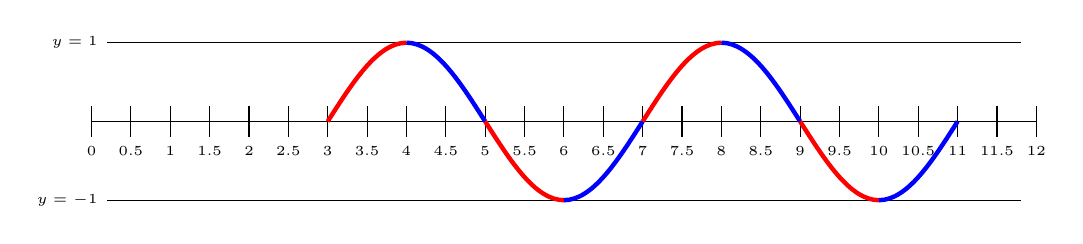
\begin{tikzpicture}
    \draw (0,0) -- (12,0);
    \draw (0.2,1)node[left,font=\tiny] {$y=1$} -- (11.8,1);
    \draw (0.2,-1)node[left,font=\tiny] {$y=-1$} -- (11.8,-1); 
    \foreach \x in {0,0.5,...,12}{
    \draw (\x,-0.2)node [below,font=\tiny,] {\x} -- (\x,0.2) ;
    }
    \draw[ultra thick, red] (3,0) sin (4,1);    %% the real business in this line
    \draw[ultra thick, blue] (4,1) cos (5,0);    %% the real business in this line
    \draw[ultra thick, red] (5,0) sin (6,-1);    %% the real business in this line
    \draw[ultra thick, blue] (6,-1) cos (7,0);    %% the real business in this line
    \draw[ultra thick, red] (7,0)  sin (8,1);    %% the real business in this line
    \draw[ultra thick, blue] (8,1) cos (9,0);    %% the real business in this line
    \draw[ultra thick, red] (9,0) sin (10,-1);    %% the real business in this line
    \draw[ultra thick, blue] (10,-1) cos (11,0);    %% the real business in this line
    \end{tikzpicture}
\end{figure}




\section{Summary}
\label{sec:ch_3_summary}

This is a topic sentence followed by explanation, elaboration and examples to summarise the second subsection. The last sentence of this paragraph shall introduce the next paragraph. \lipsum[1]

This is a topic sentence followed by explanation, elaboration and examples to summarise the third subsection. The last sentence of this paragraph shall introduce the next paragraph. \lipsum[1]

This is a topic sentence followed by explanation, elaboration and examples to summarise the fourth subsection. The last sentence of this paragraph shall introduce the next chapter. \lipsum[1]





%*****************************************
%*****************************************
%*****************************************
%*****************************************
%*****************************************






\cleardoublepage



%*******************************************************
% This program is free software: you can redistribute it and/or modify
% it under the terms of the GNU General Public License as published by
% the Free Software Foundation, either version 3 of the License, or
% (at your option) any later version.
%
% This program is distributed in the hope that it will be useful,
% but WITHOUT ANY WARRANTY; without even the implied warranty of
% MERCHANTABILITY or FITNESS FOR A PARTICULAR PURPOSE.  See the
% GNU General Public License for more details.
%
% You should have received a copy of the GNU General Public License
% along with this program.  If not, see <http://www.gnu.org/licenses/>.
%************************************************
\chapter{This is chapter four}
\label{ch:name4}
%************************************************

\begin{flushright}
{\slshape Lorem ipsum dolor sit amet, consectetuer adipiscing.}\\
{\slshape Aenean commodo ligula eget dolor. Aenean massa.}\\
% This generate dummy text. Remove this line and replace by your quote.
\medskip
--- John Doe,\\
Unified Theory of the Important Theories,\\
{\slshape An Important Journal},\\
Vol.~123, pp.~1234--1243, Dec.~2016.\\
\end{flushright}

\bigskip


%\minitoc\nomtcpagenumbers

%\marginpar{\myTitle \myVersion}

\section{Introduction}
\label{sec:ch_4_introduction}

\citet{Berg2016} argues that this is a topic sentence followed by explanation, elaboration and examples to introduce the next three subsections. The last sentence of this paragraph shall introduce the next paragraph. \lipsum[1]

This is a topic sentence followed by explanation, elaboration and examples to introduce the next three subsections \citep{Collins2016}. The last sentence of this paragraph shall introduce the next paragraph. \lipsum[1]

\citet{Graham2016} and \citet{Grant2016} assert that this is a topic sentence followed by explanation, elaboration and examples to introduce the next three subsections. The last sentence of this paragraph shall introduce the next paragraph. \lipsum[1]

\section{First main stuff}
\label{sec:ch_4_firstmain}

This is a topic sentence followed by explanation, elaboration and examples to introduce this paragraph \citep{Haney2016}. The last sentence of this paragraph shall introduce the next paragraph. \lipsum[1]

This is a topic sentence followed by explanation, elaboration and examples to introduce this paragraph \citep{Jordan2016,Morgan2016}. The last sentence of this paragraph shall introduce the next paragraph. \lipsum[1]

This is a topic sentence followed by explanation, elaboration and examples to introduce this paragraph. The last sentence of this paragraph shall introduce the next paragraph. \lipsum[1]

\section{Second main stuff}
\label{sec:ch_4_secondmain}

This is a topic sentence followed by explanation, elaboration and examples to introduce this paragraph \citep{Scott2016}. The last sentence of this paragraph shall introduce the next paragraph. \lipsum[1]

\begin{figure}[h]
    \centering
    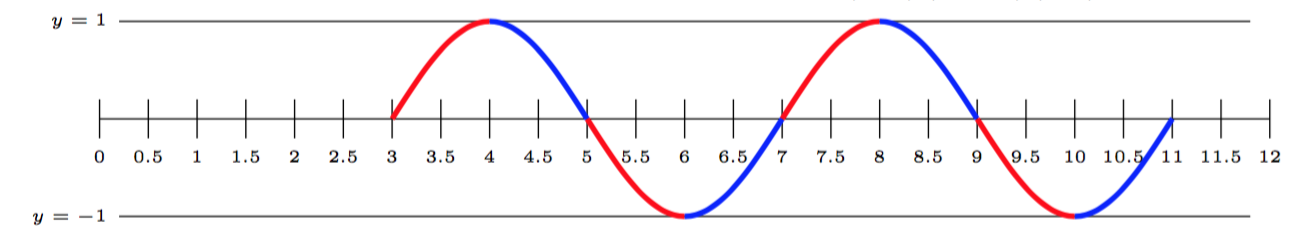
\includegraphics[width=0.9\textwidth]{imageFiles/imageExample}
    \caption{A copy from previous image}
    \label{fig:copycurve}
\end{figure}
 
As \citet{Wells2016} and \citet{Williamson2016} denotated in the figure \ref{fig:copycurve}, the 
function grows near 0. Also, in the page \pageref{fig:curve} 
is the same example in figure \ref{fig:curve}.

This is a topic sentence followed by explanation, elaboration and examples to introduce this paragraph \citep{Stewart2016}. The last sentence of this paragraph shall introduce the next paragraph. \lipsum[1]

This is a topic sentence followed by explanation, elaboration and examples to introduce this paragraph \citep{Gallagher2016}. The last sentence of this paragraph shall introduce the next paragraph. \lipsum[1]

\section{Third main stuff}
\label{sec:ch_4_thirdmain}


This is a topic sentence followed by explanation, elaboration and examples to introduce this paragraph. The last sentence of this paragraph shall introduce the next paragraph. \lipsum[1]

This is a topic sentence followed by explanation, elaboration and examples to introduce this paragraph. The last sentence of this paragraph shall introduce the next paragraph. \lipsum[1]

This is a topic sentence followed by explanation, elaboration and examples to introduce this paragraph. The last sentence of this paragraph shall introduce the next paragraph. \lipsum[1]

\section{Summary}
\label{sec:ch_4_summary}


This is a topic sentence followed by explanation, elaboration and examples to summarise the second subsection. The last sentence of this paragraph shall introduce the next paragraph. \lipsum[1]

This is a topic sentence followed by explanation, elaboration and examples to summarise the third subsection. The last sentence of this paragraph shall introduce the next paragraph. \lipsum[1]

This is a topic sentence followed by explanation, elaboration and examples to summarise the fourth subsection. The last sentence of this paragraph shall introduce the next chapter. \lipsum[1]



%*****************************************
%*****************************************
%*****************************************
%*****************************************
%*****************************************






\cleardoublepage



%*******************************************************
% This program is free software: you can redistribute it and/or modify
% it under the terms of the GNU General Public License as published by
% the Free Software Foundation, either version 3 of the License, or
% (at your option) any later version.
%
% This program is distributed in the hope that it will be useful,
% but WITHOUT ANY WARRANTY; without even the implied warranty of
% MERCHANTABILITY or FITNESS FOR A PARTICULAR PURPOSE.  See the
% GNU General Public License for more details.
%
% You should have received a copy of the GNU General Public License
% along with this program.  If not, see <http://www.gnu.org/licenses/>.
%************************************************
\chapter{This is chapter five}
\label{ch:name5}
%************************************************

\begin{flushright}
{\slshape Lorem ipsum dolor sit amet, consectetuer adipiscing.}\\
{\slshape Aenean commodo ligula eget dolor. Aenean massa.}\\
% This generate dummy text. Remove this line and replace by your quote.
\medskip
--- John Doe,\\
Unified Theory of the Important Theories,\\
{\slshape An Important Journal},\\
Vol.~123, pp.~1234--1243, Dec.~2016.\\
\end{flushright}

\bigskip


%\minitoc\nomtcpagenumbers

%\marginpar{\myTitle \myVersion}

\section{Introduction}
\label{sec:ch_5_introduction}


This is a topic sentence followed by explanation, elaboration and examples to introduce the next three subsections. The last sentence of this paragraph shall introduce the next paragraph. \lipsum[1]

This is a topic sentence followed by explanation, elaboration and examples to introduce the next three subsections. The last sentence of this paragraph shall introduce the next paragraph. \lipsum[1]

This is a topic sentence followed by explanation, elaboration and examples to introduce the next three subsections. The last sentence of this paragraph shall introduce the next paragraph. \lipsum[1]

\section{First main stuff}
\label{sec:ch_5_firstmain}

This is a topic sentence followed by explanation, elaboration and examples to introduce this paragraph. The last sentence of this paragraph shall introduce the next paragraph. \lipsum[1]

This is a topic sentence followed by explanation, elaboration and examples to introduce this paragraph. The last sentence of this paragraph shall introduce the next paragraph. \lipsum[1]

This is a topic sentence followed by explanation, elaboration and examples to introduce this paragraph. The last sentence of this paragraph shall introduce the next paragraph. \lipsum[1]

\section{Second main stuff}
\label{sec:ch_5_secondmain}

This is a topic sentence followed by explanation, elaboration and examples to introduce this paragraph. The last sentence of this paragraph shall introduce the next paragraph. \lipsum[1]

This is a topic sentence followed by explanation, elaboration and examples to introduce this paragraph. The last sentence of this paragraph shall introduce the next paragraph. \lipsum[1]

This is a topic sentence followed by explanation, elaboration and examples to introduce this paragraph. The last sentence of this paragraph shall introduce the next paragraph. \lipsum[1]

\section{Third main stuff}
\label{sec:ch_5_thirdmain}

This is a topic sentence followed by explanation, elaboration and examples to introduce this paragraph. The last sentence of this paragraph shall introduce the next paragraph. \lipsum[1]

This is a topic sentence followed by explanation, elaboration and examples to introduce this paragraph. The last sentence of this paragraph shall introduce the next paragraph. \lipsum[1]

This is a topic sentence followed by explanation, elaboration and examples to introduce this paragraph. The last sentence of this paragraph shall introduce the next paragraph. \lipsum[1]

\section{Summary}
\label{sec:ch_5_summary}


This is a topic sentence followed by explanation, elaboration and examples to summarise the second subsection. The last sentence of this paragraph shall introduce the next paragraph. \lipsum[1]

This is a topic sentence followed by explanation, elaboration and examples to summarise the third subsection. The last sentence of this paragraph shall introduce the next paragraph. \lipsum[1]

This is a topic sentence followed by explanation, elaboration and examples to summarise the fourth subsection. The last sentence of this paragraph shall introduce the next chapter. \lipsum[1]




%*****************************************
%*****************************************
%*****************************************
%*****************************************
%*****************************************






\cleardoublepage



%*******************************************************
% This program is free software: you can redistribute it and/or modify
% it under the terms of the GNU General Public License as published by
% the Free Software Foundation, either version 3 of the License, or
% (at your option) any later version.
%
% This program is distributed in the hope that it will be useful,
% but WITHOUT ANY WARRANTY; without even the implied warranty of
% MERCHANTABILITY or FITNESS FOR A PARTICULAR PURPOSE.  See the
% GNU General Public License for more details.
%
% You should have received a copy of the GNU General Public License
% along with this program.  If not, see <http://www.gnu.org/licenses/>.
%************************************************
\chapter{Conclusion}
\label{ch:conclusion}
%************************************************

\begin{flushright}
{\slshape Lorem ipsum dolor sit amet, consectetuer adipiscing.}\\
{\slshape Aenean commodo ligula eget dolor. Aenean massa.}\\
% This generate dummy text. Remove this line and replace by your quote.
\medskip
--- John Doe,\\
Unified Theory of the Important Theories,\\
{\slshape An Important Journal},\\
Vol.~123, pp.~1234--1243, Dec.~2016.\\
\end{flushright}

\bigskip

\section{Introduction}
\label{sec:ch_6_introduction}

This is a topic sentence followed by explanation, elaboration and examples to summarise chapter 2. The last sentence of this paragraph shall introduce the next paragraph. \lipsum[1]

This is a topic sentence followed by explanation, elaboration and examples for this paragraph. The last sentence of this paragraph shall introduce the next paragraph. \lipsum[1]

This is a topic sentence followed by explanation, elaboration and examples for this paragraph. The last sentence of this paragraph shall introduce the next paragraph. \lipsum[1]

\section{First main stuff}
\label{sec:ch_6_firstmain}

This is a topic sentence followed by explanation, elaboration and examples to summarise chapter 3. The last sentence of this paragraph shall introduce the next paragraph. \lipsum[1]

This is a topic sentence followed by explanation, elaboration and examples for this paragraph. The last sentence of this paragraph shall introduce the next paragraph. \lipsum[1]

This is a topic sentence followed by explanation, elaboration and examples for this paragraph. The last sentence of this paragraph shall introduce the next paragraph. \lipsum[1]

\section{Second main stuff}
\label{sec:ch_6_secondmain}

This is a topic sentence followed by explanation, elaboration and examples to summarise chapter 4. The last sentence of this paragraph shall introduce the next paragraph. \lipsum[1]

This is a topic sentence followed by explanation, elaboration and examples for this paragraph. The last sentence of this paragraph shall introduce the next paragraph. \lipsum[1]

This is a topic sentence followed by explanation, elaboration and examples for this paragraph. The last sentence of this paragraph shall introduce the next paragraph. \lipsum[1]

\section{Third main stuff}
\label{sec:ch_6_thirdmain}

This is a topic sentence followed by explanation, elaboration and examples to summarise chapter 5. The last sentence of this paragraph shall introduce the next paragraph. \lipsum[1]

This is a topic sentence followed by explanation, elaboration and examples for this paragraph. The last sentence of this paragraph shall introduce the next paragraph. \lipsum[1]

This is a topic sentence followed by explanation, elaboration and examples for this paragraph. The last sentence of this paragraph shall introduce the next paragraph. \lipsum[1]

\section{Contributions}
\label{sec:ch_6_fourthmain}

This is a topic sentence followed by explanation, elaboration and examples to summarise contributions. The last sentence of this paragraph shall introduce the next paragraph. \lipsum[1]

This is a topic sentence followed by explanation, elaboration and examples for this paragraph. The last sentence of this paragraph shall introduce the next paragraph. \lipsum[1]

This is a topic sentence followed by explanation, elaboration and examples for this paragraph. The last sentence of this paragraph shall introduce the next paragraph. \lipsum[1]

\section{Future directions}
\label{sec:ch_6_forward}

This is a topic sentence followed by explanation, elaboration and examples to summarise the above three subsections. The last sentence of this paragraph shall introduce the next paragraph. \lipsum[1]

This is a topic sentence followed by explanation, elaboration and examples for this paragraph. The last sentence of this paragraph shall introduce the next paragraph. \lipsum[1]

This is a topic sentence followed by explanation, elaboration and examples for this paragraph. The last sentence of this paragraph shall introduce the next paragraph. \lipsum[1]

This is a topic sentence followed by explanation, elaboration and examples to introduce the next chapter. The last sentence of this paragraph shall conclude the thesis. \lipsum[1]



%*****************************************
%*****************************************
%*****************************************
%*****************************************
%*****************************************






%*******************************************************
% Backmatter
%*******************************************************

\appendix



%*******************************************************
% This program is free software: you can redistribute it and/or modify
% it under the terms of the GNU General Public License as published by
% the Free Software Foundation, either version 3 of the License, or
% (at your option) any later version.
%
% This program is distributed in the hope that it will be useful,
% but WITHOUT ANY WARRANTY; without even the implied warranty of
% MERCHANTABILITY or FITNESS FOR A PARTICULAR PURPOSE.  See the
% GNU General Public License for more details.
%
% You should have received a copy of the GNU General Public License
% along with this program.  If not, see <http://www.gnu.org/licenses/>.
%************************************************
\chapter{POPLmark}
\label{ch:appendixOne}
%************************************************

\begin{flushright}
{\slshape Lorem ipsum dolor sit amet, consectetuer adipiscing.}\\
{\slshape Aenean commodo ligula eget dolor. Aenean massa.}\\
% This generate dummy text. Remove this line and replace by your quote.
\medskip
--- John Doe,\\
Unified Theory of the Important Theories,\\
{\slshape An Important Journal},\\
Vol.~123, pp.~1234--1243, Dec.~2016.\\
\end{flushright}

\bigskip

\section{Introduction}
\label{sec:ch_1_introduction}

This is a topic sentence followed by explanation, elaboration and examples to introduce the next three subsections. The last sentence of this paragraph shall introduce the next paragraph. \lipsum[1]

This is a topic sentence followed by explanation, elaboration and examples to introduce the next three subsections. The last sentence of this paragraph shall introduce the next paragraph. \lipsum[1]

This is a topic sentence followed by explanation, elaboration and examples to introduce the next three subsections. The last sentence of this paragraph shall introduce the next paragraph. \lipsum[1]

\section{First main stuff}
\label{sec:ch_1_firstmain}

This is a topic sentence followed by explanation, elaboration and examples to introduce this paragraph. The last sentence of this paragraph shall introduce the next paragraph. \lipsum[1]

This is a topic sentence followed by explanation, elaboration and examples to introduce this paragraph. The last sentence of this paragraph shall introduce the next paragraph. \lipsum[1]

This is a topic sentence followed by explanation, elaboration and examples to introduce this paragraph. The last sentence of this paragraph shall introduce the next paragraph. \lipsum[1]

\section{Second main stuff}
\label{sec:ch_1_secondmain}

This is a topic sentence followed by explanation, elaboration and examples to introduce this paragraph. The last sentence of this paragraph shall introduce the next paragraph. \lipsum[1]

This is a topic sentence followed by explanation, elaboration and examples to introduce this paragraph. The last sentence of this paragraph shall introduce the next paragraph. \lipsum[1]

This is a topic sentence followed by explanation, elaboration and examples to introduce this paragraph. The last sentence of this paragraph shall introduce the next paragraph. \lipsum[1]

\section{Third main stuff}
\label{sec:ch_1_thirdmain}


This is a topic sentence followed by explanation, elaboration and examples to introduce this paragraph. The last sentence of this paragraph shall introduce the next paragraph. \lipsum[1]

This is a topic sentence followed by explanation, elaboration and examples to introduce this paragraph. The last sentence of this paragraph shall introduce the next paragraph. \lipsum[1]

This is a topic sentence followed by explanation, elaboration and examples to introduce this paragraph. The last sentence of this paragraph shall introduce the next paragraph. \lipsum[1]

\section{Summary}
\label{sec:append_1_summary}


This is a topic sentence followed by explanation, elaboration and examples to summarise the second subsection. The last sentence of this paragraph shall introduce the next paragraph. \lipsum[1]

This is a topic sentence followed by explanation, elaboration and examples to summarise the third subsection. The last sentence of this paragraph shall introduce the next paragraph. \lipsum[1]

This is a topic sentence followed by explanation, elaboration and examples to summarise the fourth subsection. The last sentence of this paragraph shall introduce the next chapter. \lipsum[1]



%*****************************************
%*****************************************
%*****************************************
%*****************************************
%*****************************************






\cleardoublepage



%*******************************************************
% This program is free software: you can redistribute it and/or modify
% it under the terms of the GNU General Public License as published by
% the Free Software Foundation, either version 3 of the License, or
% (at your option) any later version.
%
% This program is distributed in the hope that it will be useful,
% but WITHOUT ANY WARRANTY; without even the implied warranty of
% MERCHANTABILITY or FITNESS FOR A PARTICULAR PURPOSE.  See the
% GNU General Public License for more details.
%
% You should have received a copy of the GNU General Public License
% along with this program.  If not, see <http://www.gnu.org/licenses/>.
%************************************************
\chapter{K-server problem}
\label{ch:appendixTwo}
%************************************************

\begin{flushright}
{\slshape Lorem ipsum dolor sit amet, consectetuer adipiscing.}\\
{\slshape Aenean commodo ligula eget dolor. Aenean massa.}\\
% This generate dummy text. Remove this line and replace by your quote.
\medskip
--- John Doe,\\
Unified Theory of the Important Theories,\\
{\slshape An Important Journal},\\
Vol.~123, pp.~1234--1243, Dec.~2016.\\
\end{flushright}

\bigskip


\section{Introduction}
\label{sec:ch_1_introduction}

This is a topic sentence followed by explanation, elaboration and examples to introduce the next three subsections. The last sentence of this paragraph shall introduce the next paragraph. \lipsum[1]

This is a topic sentence followed by explanation, elaboration and examples to introduce the next three subsections. The last sentence of this paragraph shall introduce the next paragraph. \lipsum[1]

This is a topic sentence followed by explanation, elaboration and examples to introduce the next three subsections. The last sentence of this paragraph shall introduce the next paragraph. \lipsum[1]

\section{First main stuff}
\label{sec:ch_1_firstmain}

This is a topic sentence followed by explanation, elaboration and examples to introduce this paragraph. The last sentence of this paragraph shall introduce the next paragraph. \lipsum[1]

This is a topic sentence followed by explanation, elaboration and examples to introduce this paragraph. The last sentence of this paragraph shall introduce the next paragraph. \lipsum[1]

This is a topic sentence followed by explanation, elaboration and examples to introduce this paragraph. The last sentence of this paragraph shall introduce the next paragraph. \lipsum[1]

\section{Second main stuff}
\label{sec:ch_1_secondmain}

This is a topic sentence followed by explanation, elaboration and examples to introduce this paragraph. The last sentence of this paragraph shall introduce the next paragraph. \lipsum[1]

This is a topic sentence followed by explanation, elaboration and examples to introduce this paragraph. The last sentence of this paragraph shall introduce the next paragraph. \lipsum[1]

This is a topic sentence followed by explanation, elaboration and examples to introduce this paragraph. The last sentence of this paragraph shall introduce the next paragraph. \lipsum[1]

\section{Third main stuff}
\label{sec:ch_1_thirdmain}


This is a topic sentence followed by explanation, elaboration and examples to introduce this paragraph. The last sentence of this paragraph shall introduce the next paragraph. \lipsum[1]

This is a topic sentence followed by explanation, elaboration and examples to introduce this paragraph. The last sentence of this paragraph shall introduce the next paragraph. \lipsum[1]

This is a topic sentence followed by explanation, elaboration and examples to introduce this paragraph. The last sentence of this paragraph shall introduce the next paragraph. \lipsum[1]

\section{Summary}
\label{sec:append_2_summary}


This is a topic sentence followed by explanation, elaboration and examples to summarise the second subsection. The last sentence of this paragraph shall introduce the next paragraph. \lipsum[1]

This is a topic sentence followed by explanation, elaboration and examples to summarise the third subsection. The last sentence of this paragraph shall introduce the next paragraph. \lipsum[1]

This is a topic sentence followed by explanation, elaboration and examples to summarise the fourth subsection. The last sentence of this paragraph shall introduce the next chapter. \lipsum[1]



%*****************************************
%*****************************************
%*****************************************
%*****************************************
%*****************************************






\cleardoublepage


%*******************************************************
% Other Stuff in the Back
%*******************************************************
\cleardoublepage

%\bibliographystyle{plainnat}
%\bibliographystyle{plain}
\bibliographystyle{apalike}

%\label{app:bibliography} 
\bibliography{exampleBibliography}

%\include{backMatters/bibliography}
%\cleardoublepage\include{FrontBackmatter/Colophon}

%*******************************************************

\end{document}

%*******************************************************
% This is the end of the thesis
%*******************************************************









